%!TEX root = ../thesis.tex

\chapter{FMM-BEM Implementation Details}
\label{chapter:fmm_implementation}
\thispagestyle{myheadings}

\graphicspath{{FMM_Implementation/}}

We have previously discussed the concepts of the {\fmm} (\S\ref{sec:fmm}) and {\bem} (\S\ref{sec:bem}), and some of the numerical techniques we will be using (\S\ref{subsec:numerical_integration}). We now  discuss implementation specifics for the {\fmm}, and in particular, specifics for the {\fmmbem}.

\section{Data Types}\label{sec:fmm_data_types}

The types of data we will deal with in the {\fmmbem}, and how we handle them is very important. We will summarize the important types that we will deal with in both {\fmm} and {\fmmbem}, highlighting the differences.

\begin{itemize}
\item \lstinline|point_type| -- A $d$-dimensional point in space, $\vect{x} \in \R^{d}$.
\item \lstinline|source_type| -- A source for the evaluation. For instance, a planetary body in astrophysics, a point vortex in vortex methods.
\item \lstinline|target_type| -- A target for the evaluation -- this can be the same as a source or simply a point in space, depending on the type of system being evaluated.
\item \lstinline|multipole_type| -- Type of the multipole expansions, e.g. a vector of complex numbers (Spherical harmonics expansions) or real numbers (cartesian expansions)
\item \lstinline|local_type| -- Analogous to \lstinline|multipole_type| for the {\fmm}'s local expansions.
\end{itemize}

Before we explicitly set these types, we can gain insight into what they might look like by thinking about the nature of what we are solving in an {\fmmbem} problem.

First, we are approximating a matrix from values on a discretized surface mesh, where each element contributes a term based on an integral over its surface with respect to a target surface. This implies that our \lstinline|source_type| is not going to be a point in space, but rather some kind of panel. It will then be easiest to represent each target as a panel too, even though we will only care about the central point in a collocation {\bem} --- this gives us the advantage of having sources and targets the same, simplifying the {\fmm} evaluations. Next, each panel can contribute one of 2 types of value -- fixed potential or charge in the case of Laplace, velocity or traction for Stokes and displacement or traction force for linear elasticity problems. Approximations to these different contributions must be kept separate, implying we should have a pair of expansions, one for each type of boundary condition.


The first {\bem}-specific change we make, is to consider a panel-type to serve as our source and target-types. Represented (at a minimum) as a set of vertices $(v_1,v_2,v_3)$, the actual implementation of the panel is irrelevant so long as standard information can be obtained from it -- quadrature points, area, normal etc. These panels will require implementation-specific {\ptop}, {\ptom} routines, and potentially {\mtop} and {\ltop} as well. An example of the code description for a constant triangle is shown below

\begin{lstlisting}
// Constant triangular panel
struct ConstantTriangle
{
  // important values
  double area;
  Point3D normal;
  // pre-computed quadrature points for triangle
  vector<Point3D> quadrature_points;
  BoundaryConditionType BC;

  // create Panel from 3 vertices
  Panel(Point3D v1, Point3D v2, Point3D v3);
  
  
  // create Panel from existing panel
  Panel(Panel other);
};
\end{lstlisting}

The change for multipole and local types is much each easier -- if we consider (in \cpp notation) a single multipole to have type {\lstinline|multipole_type|}, then the {\bem} specific type would be either {\lstinline|multipole_type[2]|}, or {\lstinline|std::vector<multipole_type>|}.

Table \ref{tab:fmm_data_types} summarizes the changes in types between the {\fmm} for a particular equation, in this case Laplace, and the {\fmmbem}.

\begin{table}[htdp]
\begin{center}
\begin{tabular}{c|c|c}
	Data type & {\fmm} & {\fmmbem} \\
	& & \\ \hline
	& & \\
	point\_type & {\lstinline|Point3D|} & {\lstinline|Point3D|} \\ 
	& & \\
	source\_type & {\lstinline|Point3D|} & {\lstinline|Panel|} \\
	& & \\
	target\_type & {\lstinline|Point3D|} & {\lstinline|Panel|} \\
	& & \\
	multipole\_type & {\lstinline|vector<complex>|} & {\lstinline|vector<complex>[2]|} \\
	& & \\
	local\_type & {\lstinline|vector<complex>|} & {\lstinline|vector<complex>[2]|}
\end{tabular}
\end{center}
\caption{Data types for Laplace {\fmm} and {\fmmbem}}
\label{tab:fmm_data_types}
\end{table}%

\section{FMM Operators}\label{sec:fmm_operators}

We have already discussed how the data types change from {\fmm} to {\fmmbem}, now we look at how the {\fmm} operators must change to accommodate these typing changes. The first operator we will look at is {\ptop}, the interaction between a single source and single target. This is generating the element $(i,j)$ if we were to form a full-rank matrix. For the {\bem}, this is calculated with

\begin{equation}
	\K(i,j) = \int_{\Gamma_j} f(\vect{x}_i, \vect{x}_j) \di{\Gamma},
\end{equation}

with $\vect{x}_i$ within the target panel, and $\vect{x}_j$ within the source. For the singular case, $i=j$, we use specific routines (see \S\ref{subsec:numerical_integration}) and Gauss quadrature for all other cases. Thus a panel need simply provide some way of accessing it's relevant quadrature points, whether explicitly storing them, or calculating on-the-fly.

Next, we look at {\ptom} - this calculates the multipole approximation from a single panel at some arbitrary point. For panels, this is as easy as iterating over the component quadrature points of each panel, treating each of them as a single source would be in a standard {\fmm}.

Translation operators, {\mtom}, {\mtol} and {\ltol} area identical to the {\fmm} counterparts, with the exception that every translation is done twice --- once for each type of boundary condition.

Finally, the evaluation operators, {\mtop} and {\ltop} will change based on the exact implementation of the panel. For constant panels, they will be identical to the {\fmm} case, with a single point being evaluating at the center of the target panel. For more complex formulations, they may require exposing more target points, rendering the situation analogous to that for {\ptom} -- the panel exposes multiple points, each of which are evaluated individually as a single point.

\section{Near-Field Sparse-Matrix}\label{sec:fmm_near_field}

One of the major advantages of using the {\fmm} to form an approximation of the full-rank {\bem} matrix, is to reduce the overall memory consumption by never explicitly storing the matrix. However, we can trade-off some of these memory savings in order to make our matrix-vector products faster. We do this by explicitly constructing the matrix of only the near-field interactions. This allows us to only perform the near-field calculation (all of the integrals) once, as each further calculation becomes a simple matrix-vector product. This is the same as calculating $A_{\text{local}}$ from \S\ref{subsec:preconditioners}, but instead of using the matrix as a preconditioner, we store it and use it instead of re-evaluating the near-field every solver iteration.

To save memory, we use the {\csr} sparse-matrix format, which consists of 3 arrays --- offsets corresponding to the beginning and end of rows, which reference to segments of the other 2 arrays, containing the column index and value of every non-zero value. An example matrix and corresponding {\csr} representation is shown below.

\begin{equation}
	A = \left(\begin{array}{ccc}
		1 & 2 & 0 \\
		0 & 1 & 0 \\
		3 & 0 & 1
	\end{array}\right)
\end{equation}

\begin{table}[h]
\begin{center}
\begin{tabular}{c|ccccc}
	offsets & 0 & 2 & 3 & 5 & \\
	 & & & & & \\
	indices & 0 & 1 & 1 & 0 & 2 \\
	 & & & & & \\
	values & 1 & 2 & 1 & 3 & 1
\end{tabular}
\end{center}
\caption{{\csr} representation of $A$}
\end{table}%

In the case of the near-field, every row corresponds to a source panel, and every column entry signifies a direct (\ptop) interaction between the source and that target. The total storage for this matrix form in double precision is: $(\# \text{rows} \times 4) + (\text{nnz} \times 12)\;\text{bytes}$ . While this form of near-field interaction can be used for a standard {\fmm}, it can cause some notable problems:

\begin{itemize}
\item If sources move, the sparse-matrix has to be re-created, including the non-zero (sparsity) pattern -- there are no corresponding savings for multiple iterations.
\item In uniform distributions of sources, each individual source will on average interact with  $27\times\ncrit$ other particles, resulting in very memory-intensive matrices. For instance, $N = 10^{4},\;\ncrit=400$ would result in a matrix taking 1236MB. Increasing $N$ to $10^{5}$ would give a matrix taking 12.36GB. We can use this technique more readily for {\bem} applications, as the nature of the surface mesh will result in less than 27 near-field cluster-cluster interactions, reducing that number to around 9, with an equivalent reduction in memory consumption.
\end{itemize}

\section{Lazy Evaluators}\label{sec:fmm_lazy_eval}

In the {\fmmbem}, we have the advantage that once we create the spatial decomposition of the domain, it doesn't change throughout the iterations of the linear solve. This means we can traverse the tree a single time, storing the resulting interactions in lists, and simply run through those lists once for every iteration.For example, the upward sweep shown in algorithm \ref{alg:upward_sweep} turns into algorithm \ref{alg:upward_sweep_lazy} when performed in a lazy fashion.

Analogous variations on algorithms \ref{alg:interaction} and \ref{alg:downward_sweep} can also be created.

\begin{algorithm}
	\caption{Lazy Upward sweep}
	\label{alg:upward_sweep_lazy}
	\begin{algorithmic}
		\Require Cells $C$, kernel $K$.
		\State P2M\_list = []
		\State M2M\_list = []
		\State // Once during construction
		\For{i=1,\;...,\;\Call{size}{$C$}}
			\If{\Call{is\_leaf}{$C_{i}$}} 
				\State \Call{p2m\_list.insert}{i} \Comment Queue P2M operation for leaf
			\Else
				\State p = \Call{pair}{i, parent($C_{i}$).index} \Comment Queue M2M operation up tree
				\State \Call{m2m\_list.insert}{p}
			\EndIf
		\EndFor
		\State // Each Iteration
		\For{Entries $i$ in P2M\_list}
			\State \Call{k.p2m}{$C_i$} \Comment Evaluate queued P2M
		\EndFor
		\For{Entries $i$ in M2M\_list}
			\State \Call{k.m2m}{$C_{\text{i.first}},\;C_{\text{i.second}}$} \Comment Evaluate queued M2M
		\EndFor
	\end{algorithmic}
\end{algorithm}

A further advantage to this style of evaluation beyond saving the cost of repeated tree traversals, is that we can process lists of queued operations in parallel very easily. The most obvious candidates for this treatment are lists for {\ptom} and {\ltop}, where every operator call only involves a single cell, and every cell is completely independent. All other lists can still be performed in parallel, albeit with more care taken to ensure no race conditions (multiple parallel processes attempting to change the same value(s) simultaneously) occur.

\section{Performance}\label{sec:fmm_performance}

While we have asserted in \S\ref{sec:fmm} that the {\fmm} scales as $\O{N}$, we should confirm that our implementation scales correctly. All kernels should scale equally, so we choose to use the Laplace kernel, utilizing spherical harmonic expansions, with $p = 5$. We choose to keep $\ncrit = 126$ for all cases, and values of $N$ are chosen such that all data points are equispaced on a log-log plot, shown below in figure \ref{fig:fmm_scaling}.

%We will adjust $\ncrit$ to ensure that the traditional equal balance of near and far-fields is maintained. 

\begin{figure}[h]
\begin{center}
	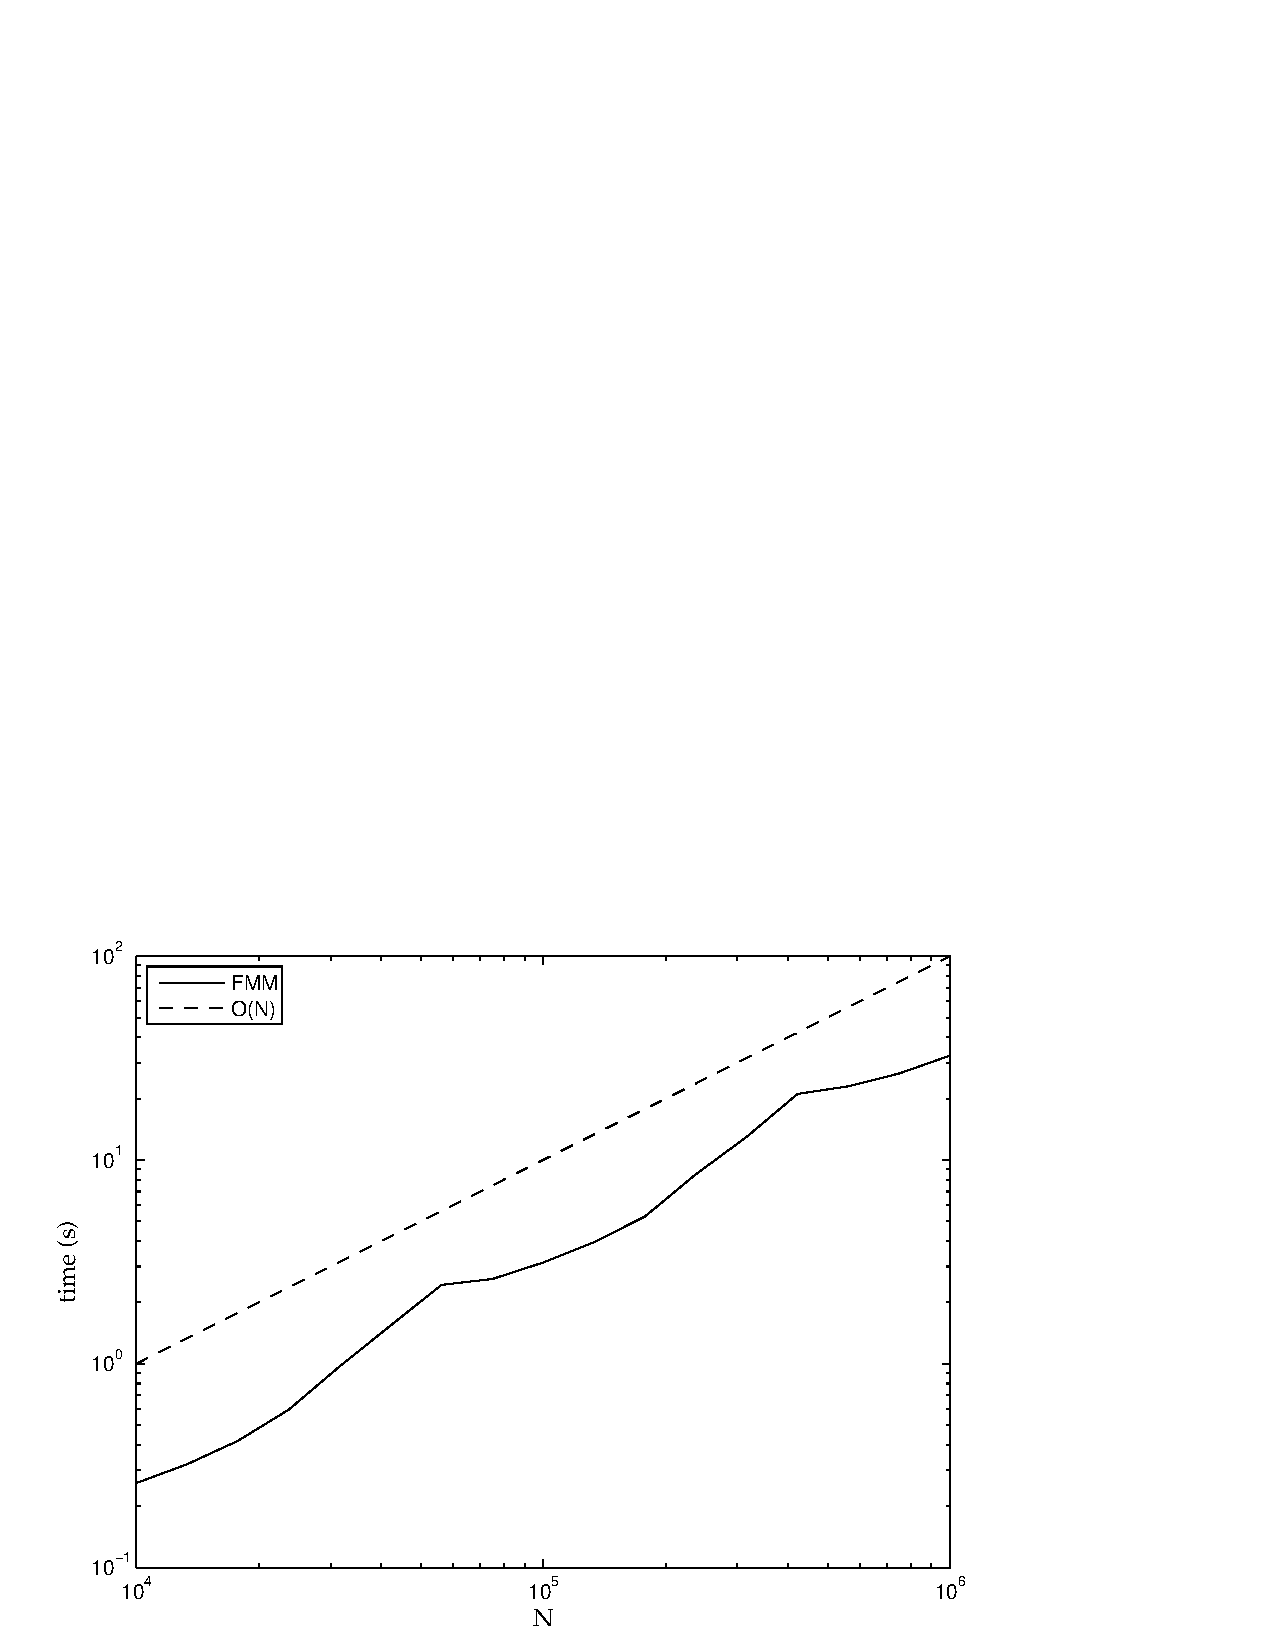
\includegraphics[width=14cm]{img/FMMScaling.pdf}
	\caption{Scaling of the {\fmm} with respect to problem size, $N$}
	\label{fig:fmm_scaling}
\end{center}
\end{figure}

This plot shows the overall scaling of the {\fmm} as $\O{N}$. The minor peaks are caused by the nature of the hierarchical decomposition -- when a new level is added it changes the balance of near and far-field computation, which is vital to the overall $\O{N}$ behavior. We could eliminate these peaks by tweaking $\ncrit$ for every test value of $N$, but the general trend of timing has already been shown.